\begin{frame}
    \titlepage
\end{frame}

\tikzset{
    stackBox/.style={very thick},
    allocBox/.style={dashed,very thick,fill=blue!20},
    onStack/.style={thick},
    frameOne/.style={fill=blue!15},
    frameTwo/.style={fill=red!15},
    markLine/.style={blue!50!black},
    markLineB/.style={red!90!black},
    hiLine/.style={red!90!black},
}

\begin{frame}{last time}
    \begin{itemize}
            \item stack canaries
            \begin{itemize}
                \item less-compatible alternative: shadow stacks
            \end{itemize}
            \item page-level protection
                \begin{itemize}
                \item RELRO --- protect global offset table
                \item guard pages around memory allocations/etc.
                \end{itemize}
            \item start ASLR
                \begin{itemize}
                \item choose random addresses
                \item ideally attacker never learns addresses
                    \begin{itemize}
                    \item except overflows can leak them
                    \end{itemize}
                \end{itemize}
    \end{itemize}
\end{frame}

\begin{frame}{logistical note: FORMAT}
    \begin{itemize}
    \item deadline Saturday 
    \begin{itemize}\item since executable was not linked correctly on time\end{itemize}
    \item format string exploit
        \begin{itemize}
        \item sufficient to overwrite \texttt{defaultLetterGrade} variable
        \end{itemize}
    \end{itemize}
\end{frame}

\begin{frame}<0>[fragile,label=aslr64]{program memory (x86-64 Linux; ASLR)}
\begin{tikzpicture}[remember picture]
\tikzset{
    mylabel/.style={font=\ttfamily,align=center,append after command={([xshift=.1cm]\tikzlastnode.west) edge[ultra thick] ++(-.2cm,0cm)}},
    mybox/.style={draw,rectangle,minimum width=7cm,fill=white},
    myhigh/.style={draw,rectangle,line width=1mm, draw=blue!80!black,opacity=.3},
}
\node[mybox,minimum height=.5cm,inner ysep=0mm,pattern=north west lines,pattern color=black!50!white] (kernel) {Used by OS};
\begin{pgfonlayer}{bg}
    \node[right=1mm of kernel.north east,mylabel] (topLabel) {0xFFFF FFFF FFFF FFFF};
    \node[right=1mm of kernel.south east,mylabel] {0xFFFF 8000 0000 0000};
\end{pgfonlayer}
\node[mybox, minimum height=.5cm, below=.45cm of kernel] (stack) {Stack};
\begin{pgfonlayer}{bg}
    \node[right=1mm of stack.north east,mylabel] {\myemph<1>{$\pm$ 0x004 0000 0000}};
\end{pgfonlayer}
\node[mybox, minimum height=.5cm, below=0.5cm of stack] (heapB) {Dynamic/Libraries (mmap)};
\begin{pgfonlayer}{bg}
    \node[right=1mm of heapB.north east,mylabel] (heapBLabel) {\myemph<1>{$\pm$ 0x100 0000 0000}};
    \node[below=0mm of heapBLabel,font=\small,inner sep=0mm] {(filled from top with ASLR)};
\end{pgfonlayer}
%\begin{pgfonlayer}{bg}
%    \node[right=1mm of heapB.south east,mylabel] (heapBLabel) {0x0000 2baa aaaa b000 \\ $\pm$ 0x100 0000 0000\*};
%\end{pgfonlayer}
\node[mybox, minimum height=.5cm, below=0.5cm of heapB] (heap) {Heap (brk/sbrk)};
\begin{pgfonlayer}{bg}
\node[right=1mm of heap.south east,mylabel] (heapBLabel) {\myemph<1>{$\pm$ 0x200 0000}};
\end{pgfonlayer}
\node[mybox, minimum height=.5cm, below=0.2mm of heap] (data) {Writable data};
\begin{pgfonlayer}{bg}
\node[right=1mm of data.south east,mylabel] (bottomLabel) {\myemph<2-3>{0x0000 0000 0060 0000}*};
\node[below=0mm of bottomLabel,font=\small,inner sep=0mm] {(constants + 2MB alignment)};
\end{pgfonlayer}
\node[mybox, minimum height=.5cm, below=0.6cm of data] (sdata) {Code + Constants};
\begin{pgfonlayer}{bg}
\node[right=1mm of sdata.south east,mylabel] (sbottomLabel) {\myemph<2-3>{0x0000 0000 0040 0000}};
\end{pgfonlayer}
\coordinate (memBottom) at ($(sdata.south east) + (0mm, -2mm)$);
\begin{pgfonlayer}{bg}
\draw[pattern=north west lines, pattern color=black!40!white] (kernel.north west) rectangle (memBottom);
\end{pgfonlayer}

\begin{visibleenv}<3>
    \begin{scope}[overlay]
    \node[draw=red,ultra thick,fill=white,anchor=center,
          inner sep=.5cm,font=\Large] at (current page.center) {
        why are these addresses fixed?
    }; 
    \end{scope}
\end{visibleenv}

\end{tikzpicture}
\end{frame}
\begin{frame}<0>[label=mappingList]{the mapping (set by OS)}
\begin{tikzpicture}
\tikzset{
    dot/.style={draw=none}
}
\matrix[tight matrix,nodes={minimum height=.525cm,text width=3cm,font=\small\tt},
    row 1/.style={nodes={font=\bfseries\small\normalfont}},
    column 1/.style={nodes={draw=none,text width=6cm}},
    column 2/.style={nodes={text width=1cm}},
    column 3/.style={nodes={text width=1cm}},
    column 4/.style={nodes={alt=<2>{opacity=1.0,red}{opacity=0.0},text width=1cm}},
] {
program address range \& read? \& write? \& exec? \& real address\\
0x0000 --- 0x0FFF \& no \& no \& no \& --- \\
0x1000 --- 0x1FFF \& no \& no \& no \& --- \\
|[dot]| \ldots \\
0x40 0000 --- 0x40 0FFF \& yes \& no \& yes \& 0x... \\
0x40 1000 --- 0x40 1FFF \& yes \& no \& yes \& 0x... \\
0x40 2000 --- 0x40 2FFF \& yes \& no \& yes \& 0x... \\
|[dot]| \ldots \\
0x60 0000 --- 0x60 0FFF \& yes \& yes \& no\& 0x... \\
0x60 1000 --- 0x60 1FFF \& yes \& yes \& no\& 0x... \\
|[dot]| \ldots \\
|[font=\scriptsize]| 0x7FFF FF00 0000 --- 0x7FFF FF00 0FFF \& yes \& yes \& no\& 0x... \\
|[font=\scriptsize]| 0x7FFF FF00 1000 --- 0x7FFF FF00 1FFF \& yes \& yes \& no\& 0x... \\
|[dot]| \ldots \\
};
\end{tikzpicture}
\end{frame}

\section{ASLR}

\subsection{How much entropy?}

\begin{frame}{Linux stack randomization (x86-64)}
\begin{itemize}
    \item 1. choose random number between \texttt{0} and \tikzmark{range}\myemph<2>{\texttt{0x3F FFFF}}
    \item 2. stack starts at \texttt{0x7FFF FFFF FFFF} - \textit{random number} $\times$ \texttt{0x1000}
        \begin{itemize}
        \item randomization disabled? \textit{random number} $= 0$
        \end{itemize}
\end{itemize}
\begin{tikzpicture}[overlay,remember picture]
\node[mycallout=range] at ([yshift=-1cm]current page.center) {
    16 GB range!
};
\end{tikzpicture}
\end{frame}

\begin{frame}<1>[fragile,label=aslr64]{program memory (x86-64 Linux; ASLR)}
\begin{tikzpicture}[remember picture]
\tikzset{
    mylabel/.style={font=\ttfamily,align=center,append after command={([xshift=.1cm]\tikzlastnode.west) edge[ultra thick] ++(-.2cm,0cm)}},
    mybox/.style={draw,rectangle,minimum width=7cm,fill=white},
    myhigh/.style={draw,rectangle,line width=1mm, draw=blue!80!black,opacity=.3},
}
\node[mybox,minimum height=.5cm,inner ysep=0mm,pattern=north west lines,pattern color=black!50!white] (kernel) {Used by OS};
\begin{pgfonlayer}{bg}
    \node[right=1mm of kernel.north east,mylabel] (topLabel) {0xFFFF FFFF FFFF FFFF};
    \node[right=1mm of kernel.south east,mylabel] {0xFFFF 8000 0000 0000};
\end{pgfonlayer}
\node[mybox, minimum height=.5cm, below=.45cm of kernel] (stack) {Stack};
\begin{pgfonlayer}{bg}
    \node[right=1mm of stack.north east,mylabel] {\myemph<1>{$\pm$ 0x004 0000 0000}};
\end{pgfonlayer}
\node[mybox, minimum height=.5cm, below=0.5cm of stack] (heapB) {Dynamic/Libraries (mmap)};
\begin{pgfonlayer}{bg}
    \node[right=1mm of heapB.north east,mylabel] (heapBLabel) {\myemph<1>{$\pm$ 0x100 0000 0000}};
    \node[below=0mm of heapBLabel,font=\small,inner sep=0mm] {(filled from top with ASLR)};
\end{pgfonlayer}
%\begin{pgfonlayer}{bg}
%    \node[right=1mm of heapB.south east,mylabel] (heapBLabel) {0x0000 2baa aaaa b000 \\ $\pm$ 0x100 0000 0000\*};
%\end{pgfonlayer}
\node[mybox, minimum height=.5cm, below=0.5cm of heapB] (heap) {Heap (brk/sbrk)};
\begin{pgfonlayer}{bg}
\node[right=1mm of heap.south east,mylabel] (heapBLabel) {\myemph<1>{$\pm$ 0x200 0000}};
\end{pgfonlayer}
\node[mybox, minimum height=.5cm, below=0.2mm of heap] (data) {Writable data};
\begin{pgfonlayer}{bg}
\node[right=1mm of data.south east,mylabel] (bottomLabel) {\myemph<2-3>{0x0000 0000 0060 0000}*};
\node[below=0mm of bottomLabel,font=\small,inner sep=0mm] {(constants + 2MB alignment)};
\end{pgfonlayer}
\node[mybox, minimum height=.5cm, below=0.6cm of data] (sdata) {Code + Constants};
\begin{pgfonlayer}{bg}
\node[right=1mm of sdata.south east,mylabel] (sbottomLabel) {\myemph<2-3>{0x0000 0000 0040 0000}};
\end{pgfonlayer}
\coordinate (memBottom) at ($(sdata.south east) + (0mm, -2mm)$);
\begin{pgfonlayer}{bg}
\draw[pattern=north west lines, pattern color=black!40!white] (kernel.north west) rectangle (memBottom);
\end{pgfonlayer}

\begin{visibleenv}<3>
    \begin{scope}[overlay]
    \node[draw=red,ultra thick,fill=white,anchor=center,
          inner sep=.5cm,font=\Large] at (current page.center) {
        why are these addresses fixed?
    }; 
    \end{scope}
\end{visibleenv}

\end{tikzpicture}
\end{frame}

\begin{frame}{program memory (x86-32 Linux; ASLR)}
\begin{tikzpicture}
\tikzset{
    mylabel/.style={font=\ttfamily,align=center,append after command={([xshift=.1cm]\tikzlastnode.west) edge[ultra thick] ++(-.2cm,0cm)}},
    mybox/.style={draw,rectangle,minimum width=7cm,fill=white},
    myhigh/.style={draw,rectangle,line width=1mm, draw=blue!80!black,opacity=.3},
}
\node[mybox,minimum height=.5cm,inner ysep=0mm,pattern=north west lines,pattern color=black!50!white] (kernel) {Used by OS};
\begin{pgfonlayer}{bg}
    \node[right=1mm of kernel.north east,mylabel] (topLabel) {0xFFFF FFFF};
    \node[right=1mm of kernel.south east,mylabel] {0xC000 0000};
\end{pgfonlayer}
\node[mybox, minimum height=.5cm, below=.5cm of kernel] (stack) {Stack};
\begin{pgfonlayer}{bg}
    \node[right=1mm of stack.north east,mylabel] {\myemph{$\pm$ 0x080 0000} (default)};
\end{pgfonlayer}
\node[mybox, minimum height=.5cm, below=0.5cm of stack] (heapB) {Dynamic/Libraries (mmap)};
\begin{pgfonlayer}{bg}
    \node[right=1mm of heapB.north east,mylabel] (heapBLabel) {\myemph{$\pm$ 0x008 0000} (default)};
\end{pgfonlayer}
%\begin{pgfonlayer}{bg}
%    \node[right=1mm of heapB.south east,mylabel] (heapBLabel) {0x0000 2baa aaaa b000 \\ $\pm$ 0x100 0000 0000\*};
%\end{pgfonlayer}
\node[mybox, minimum height=.5cm, below=0.5cm of heapB] (heap) {Heap (brk/sbrk)};
\begin{pgfonlayer}{bg}
\node[right=1mm of heap.south east,mylabel] (heapBLabel) {\myemph{$\pm$ 0x200 0000}};
\end{pgfonlayer}
\node[mybox, minimum height=.5cm, below=0.2mm of heap] (data) {Writable data};
\begin{pgfonlayer}{bg}
%\node[right=1mm of data.south east,mylabel] (bottomLabel) {0x0804 0000};
\end{pgfonlayer}
\node[mybox, minimum height=.5cm, below=0.6cm of data] (sdata) {Code + Constants};
\begin{pgfonlayer}{bg}
\node[right=1mm of sdata.south east,mylabel] (bottomLabel) {0x0804 8000};
\end{pgfonlayer}
\coordinate (memBottom) at ($(sdata.south east) + (0mm, -2mm)$);
\begin{pgfonlayer}{bg}
\draw[pattern=north west lines, pattern color=black!40!white] (kernel.north west) rectangle (memBottom);
\end{pgfonlayer}
\end{tikzpicture}
\end{frame}

\begin{frame}{how much guessing?}
    \begin{itemize}
    \item gaps change by multiples of page (4K)
        \begin{itemize}
        \item lower 12 bits are \myemph{fixed}
        \end{itemize}
    \item 64-bit: \myemph{huge} ranges --- need millions of guesses
        \begin{itemize}
        \item about \myemph{30 randomized bits} in addresses
        \end{itemize}
    \item 32-bit: \myemph{smaller} ranges --- hundreds of guesses
        \begin{itemize}
        \item only about \myemph{8 randomized bits} in addresses
        \item why? only 4 GB to work with!
        \item can be configured higher --- but larger gaps
        \end{itemize}
    \end{itemize}
\end{frame}

\begin{frame}[fragile,label=noGuessing]{danger of leaking pointers}
    \begin{itemize}
        \item any stack pointer? know everything on the stack!
        \item any pointer to a particular library? know everything in library!
            \begin{itemize}
                \item library loaded as one big chunk
                \item contains many offsets in instructions --- can't split easily
            \end{itemize}
    \end{itemize}
\end{frame}

\subsection{Hard-coded addresses}

\againframe<2-3>{aslr64}

\begin{frame}{fixed addresses}
    \begin{itemize}
    \item machine code contains hard-coded addresses
    \item and is supposed to be loaded without changes
        \begin{itemize}
        \item only small global offset table, etc. changed
        \end{itemize}
    \end{itemize}
\end{frame}

\begin{frame}{one possibility --- not fixed}
    \begin{itemize}
        \item could just \myemph{edit fixed addresses at load time}
        \item usual dynamic linking strategy avoids this
            \begin{itemize}
                \item typical dynamic linkers support it, but unused by compilers, etc.
            \end{itemize}
        \item a lot slower than writing small table of addresses
        \item a lot more ``metadata'' for linker
        \item harder to share memory between programs
    \end{itemize}
\end{frame}

\begin{frame}{relocating: Windows}
    \begin{itemize}
        \item Windows will \myemph{edit code} to relocate
        \item programs/libraries \textit{usually} include \myemph{relocation table}
        \item typically one fixed location per program/library \textbf{per boot}
            \begin{itemize}
                \item same address used across all instances of program/library
                \item still allows sharing memory
            \end{itemize}
        \item fixup once per program/library per boot
            \begin{itemize}
                \item before ASLR: code could be pre-relocated
            \end{itemize}
        \item Windows + Visual Studio had `full' ASLR by default since 2010
    \end{itemize}
\end{frame}
\begin{frame}[fragile,label=reloc]{recall: relocation}
\lstset{
    language=myasm,
    style=small,
    moredelim={**[is][\btHL<1>]{~1~}{~end~}},
    moredelim={**[is][\btHL<2>]{~2~}{~end~}},
}
\begin{lstlisting}
.data
string: .asciz "Hello, World!"
.text
main:
    movq $~1~string~end~, %rdi /* NOT PC/RIP-relative mov */
\end{lstlisting}
    generates: (\texttt{objdump --disassemble --reloc})
\lstset{
    language={},
    style=small,
    moredelim={**[is][\btHL<1>]{~1~}{~end~}},
    moredelim={**[is][\btHL<2>]{~2~}{~end~}},
}
\begin{lstlisting}
   0:   48 c7 c7 00 00 00 00    mov    $0x0,%rdi
                        ~1~3: R_X86_64_32S .data~end~
\end{lstlisting}
    \begin{itemize}
        \item \myemph{relocation record} says how to fix \texttt{0x0} in \texttt{mov}
            \begin{itemize}
                \item 3: location in machine code
                \item \texttt{R\_X86\_64\_32S}: 32-bit signed integer
                \item \texttt{.data}: address to insert
            \end{itemize}
    \end{itemize}
\end{frame}

\begin{frame}{relocating and stubs: Windows}
    \begin{itemize}
        \item What about the ``stubs'' and lookup tables?
            \begin{itemize}
                \item Windows GOT equivalent is IAT (Import Address Table)
            \end{itemize}
        \item Can't Windows avoid them by editing code?
        \item Probably, but\ldots it doesn't
        \item Why?
    \end{itemize}
\end{frame}

\begin{frame}{Windows ASLR limitation}
    \begin{itemize}
        \item same address in all programs --- not very useful against local exploits
    \end{itemize}
\end{frame}

\begin{frame}{PIC: Linux, OS X}
    \begin{itemize}
        \item \myemph{position independent code}
            \begin{itemize}
                \item instead of fixed-up hard-coded addresses
            \end{itemize}
        \item Linux, OS X don't fixup code at runtime
        \item previously a challenge for ASLR
        \item libraries on these systems previously had no fixed address
        \item \ldots but executables had a bunch
    \end{itemize}
\end{frame}

\newcommand{\myemphTwo}[1]{\myemph<2>{#1}}%
\newcommand{\myemphThree}[1]{\myemph<3>{#1}}%
\newcommand{\myemphFour}[1]{\myemph<{#1}}%
\newcommand{\antiEmphThree}[1]{{\color<3>{blue}#1}}%
\newcommand{\antiEmphFour}[1]{{\color<4>{blue}#1}}%
\begin{frame}[fragile,label=hardCodedAsm]{hard-coded addresses? (64-bit)}
\lstset{language=C,style=small}
\begin{tikzpicture}
\node[anchor=north east] (code) at (-1, 0) {
\begin{lstlisting}
int foo(long n) {
    switch (n) {
    case 0: 
    case 2:
    case 4:
    case 5:
        return 1;
    case 1:
    case 3:
        return 2;
    default:
        return 3;
    }
}
\end{lstlisting}
};
\draw[thick] (-.75, 0) -- (-.75,-7);
\node[anchor=north west,align=left] (disasm) at (-.5, 0) {
\lstset{
    language=myasm,
    style=smaller,
    escapeinside=~~,
}
\begin{lstlisting}
foo:
	movl	$3, %eax
	cmpq	$5, %rdi
	ja	defaultCase
	jmp	*lookupTable(,%rdi,8)
        /* code for defaultCase, returnOne, returnTwo */
        ...
	.section	.rodata
lookupTable: /* read-only pointers: */
	.quad	returnOne
	.quad	returnTwo
	.quad	returnOne
	.quad	returnTwo
	.quad	returnOne
	.quad	returnOne
\end{lstlisting}
};
\end{tikzpicture}
\end{frame}


\begin{frame}[fragile,label=hardCodedDisasm]{hard-coded addresses? (64-bit)}
\lstset{language=C,style=small}
\begin{tikzpicture}
\node[anchor=north east] (code) at (-1, 0) {
\begin{lstlisting}
int foo(long n) {
    switch (n) {
    case 0: 
    case 2:
    case 4:
    case 5:
        return 1;
    case 1:
    case 3:
        return 2;
    default:
        return 3;
    }
}
\end{lstlisting}
};
\draw[thick] (-.75, 0) -- (-.75,-7);
\node[anchor=north west,align=left] (disasm) at (-.5, 0) {
\lstset{
    language=myasm,
    style=smaller,
    escapeinside=~~,
}
\begin{lstlisting}
~\textit{400570 <foo>}~:
b8 03 00 00 00    mov    $0x3,%eax
48 83 ff 05       cmp    $0x5,%rdi
        /* jump to defaultCase: */
77 ~\antiEmphThree{12}~            ja     ~\antiEmphThree{0x40058d}~
        /* lookup table jump: */
ff 24 fd
~\myemphTwo{18 06 40 00}~      jmpq   *~\myemphTwo{0x400618}(,\%rdi,8)~
...
 /* lookupTable @ 0x400618 */
~\textit{@ 400618:} \myemphTwo{0x400588}~ /* returnOne */
~\textit{@ 400620:} \myemphTwo{0x400582}~ /* returnTwo */
~\textit{@ 400628:} \myemphTwo{0x400588}~
~\textit{@ 400630:} \myemphTwo{0x400582}~
\end{lstlisting}
};
\end{tikzpicture}
\end{frame}

\begin{frame}[fragile,label=ex]{exercise: avoiding absolute addresses}
\lstset{
    language=myasm,
    style=smaller,
    escapeinside=~~,
}
\begin{tikzpicture}
\node[anchor=north east] (code) at (-1, 0) {
\begin{lstlisting}
foo:
	movl	$3, %eax
	cmpq	$5, %rdi
	ja	defaultCase
	jmp	*lookupTable(,%rdi,8)
returnOne:
        movl    $1, %eax
        ret
returnTwo:
        movl    $2, %eax
defaultCase:
        ret
\end{lstlisting}
};
\node[anchor=north west] (code2) at (-.5, 0) {
\begin{lstlisting}
lookupTable:
    .quad returnOne
    .quad returnTwo
    .quad returnOne
    .quad returnTwo
    .quad returnOne
    .quad returnOne
\end{lstlisting}
};
\end{tikzpicture}
\begin{itemize}
    \item exercise: rewrite this without absolute addresses
    \item but fast
\end{itemize}
\end{frame}

\begin{frame}[fragile,label=hardCodedB]{hard-coded addresses}
\begin{tikzpicture}
\node[anchor=north east] (code) at (-1, 0) {
\lstset{
    language={},
    style=smaller,
    escapeinside=~~,
}
\begin{lstlisting}
test-64-nopie.exe:     file format elf64-x86-64
test-64-nopie.exe
architecture: i386:x86-64, flags 0x00000112:
EXEC_P, HAS_SYMS, D_PAGED
start address 0x0000000000400450

Program Header:
    PHDR off    0x0000000000000040 vaddr ~\myemph{0x0000000000400040}~ paddr 0x0000000000400040 align 2**3
         filesz 0x00000000000001f8 memsz 0x00000000000001f8 flags r-x
  INTERP off    0x0000000000000238 vaddr ~\myemph{0x0000000000400238}~ paddr 0x0000000000400238 align 2**0
         filesz 0x000000000000001c memsz 0x000000000000001c flags r--
    LOAD off    0x0000000000000000 vaddr ~\myemph{0x0000000000400000}~ paddr 0x0000000000400000 align 2**21
         filesz 0x000000000000078c memsz 0x000000000000078c flags r-x
    LOAD off    0x0000000000000e10 vaddr ~\myemph{0x0000000000600e10}~ paddr 0x0000000000600e10 align 2**21
         filesz 0x0000000000000228 memsz 0x0000000000000230 flags rw-
\end{lstlisting}
};
\end{tikzpicture}
\end{frame}

\begin{frame}{relocation?}
    \begin{itemize}
        \item one solution: be willing change addresses at load time
        \item requires: table of \myemph{relocations} in \myemph{executable code}
        \item Windows does this
        \item Linux's dynamic linker is not willing to
    \end{itemize}
\end{frame}

\begin{frame}{PIE}
    \begin{itemize}
    \item position-independent executables (PIE)
        \begin{itemize}
        \item no hardcoded addresses
        \end{itemize}
    \item alternative: \myemph{edit code (not global offset table) at load time}
        \begin{itemize}
        \item Windows solution
        \end{itemize}
    \item GCC: \texttt{-pie -fPIE}
        \begin{itemize}
        \item \texttt{-pie} is linking option
        \item \texttt{-fPIE} is compilation option
        \item related option: \texttt{-fPIC} (position independent code)
            \begin{itemize}
            \item used to compile runtime-loaded libraries
            \end{itemize}
        \end{itemize}
    \end{itemize}
\end{frame}

\begin{frame}[fragile,label=PIEjtasm]{PIE jump-table}
\begin{tikzpicture}
\node[anchor=north east] (code) at (-1, 0) {
\lstset{
    language=myasm,
    style=smaller,
    escapeinside=~~,
}
\begin{lstlisting}
foo:
  movl	 $3, %eax
  cmpq	 $5, %rdi
  ja	 retDefault
  leaq	 ~\myemphTwo{jumpTable(\%rip)},~%rax
  movslq ~\myemphTwo{(\%rax,\%rdi,4)},~%rdx
  addq	 %rdx, %rax
  ~\myemphTwo{\bfseries jmp}~   ~\myemphTwo{*\%rax}~
returnTwo:
  movl  $2, %eax
  ret
returnOne:
  movl  $1, %eax
defaultCase:
  ret
\end{lstlisting}
};
\node[anchor=north west] (code2) at ([xshift=2cm]code.north east) {
\lstset{
    language={},
    style=smaller,
    escapeinside=~~,
}
\begin{lstlisting}
  .section	.rodata
jumpTable:
  .long	returnOne-jumpTable
  .long	returnTwo-jumpTable
  .long	returnOne-jumpTable
  .long	returnTwo-jumpTable
  .long	returnOne-jumpTable
  .long	returnOne-jumpTable
\end{lstlisting}
};
\end{tikzpicture}
\end{frame}

\begin{frame}[fragile,label=PIEjt]{PIE jump-table}
\begin{tikzpicture}
\node[anchor=north east] (code) at (-1, 0) {
\lstset{
    language=myasm,
    style=smaller,
    escapeinside=~~,
}
\begin{lstlisting}
~\myemphTwo{00000000000007ab}~ <foo>:
b8 03 00 00 00       	mov    $0x3,%eax
48 83 ff 05             cmp    $0x5,%rdi
77 1b                	ja     7d0 <foo+0x25>
48 8d 05 ab 00 00 00 	lea    ~\myemphThree{0xab(\%rip),}~%rax        # 868
48 63 14 b8          	movslq ~\myemphThree{(\%rax,\%rdi,4),}~%rdx
48 01 d0             	add    %rdx,%rax
ff e0                	jmpq   *%rax
b8 02 00 00 00       	mov    $0x2,%eax
c3                   	retq   
b8 01 00 00 00       	mov    $0x1,%eax
c3                	retq
...
~\textit{\myemphThree{@ 868}}:~ -156 /* offset */
~\textit{\myemphThree{@ 870}}:~ -162
...
\end{lstlisting}
};
\end{tikzpicture}
\end{frame}

\begin{frame}{added cost}
\begin{itemize}
    \item replace \texttt{jmp *jumpTable(,\%rdi,8)}
    \vspace{.5cm}
    \item with:
        \item \texttt{lea} (get table address --- with relative offset)
        \item \texttt{movslq} (do table lookup of offset)
        \item \texttt{add} (add to base)
        \item \texttt{jmp} (to computed base)
\end{itemize}

\end{frame}

\begin{frame}[fragile,label=x86Worse]{32-bit x86 is worse}
    \begin{itemize}
    \item no relative addressing for {\tt mov}, {\tt lea}, \ldots
    \item even changes ``stubs'' for printf:
    \end{itemize}
\lstset{
    language=myasm,
    style=smaller,
    escapeinside=~~,
}
\begin{lstlisting}
// BEFORE: (fixed addresses)
08048310 <__printf_chk@plt>:
 8048310: ff 25 ~\myemphTwo{10 a0 04 08}~  jmp    *0x804a010
    /* 0x804a010 == global offset table entry */

// AFTER: (position-independent)
00000490 <__printf_chk@plt>:
 490:	ff a3 10 00 00 00    jmp    *0x10~\myemphThree{(\%ebx)}~
    /* %ebx --- address of global offset table */
    /* needs to be set by caller */
\end{lstlisting}
\end{frame}

\subsection{Performance cost}

\begin{frame}{position independence cost (32-bit)}
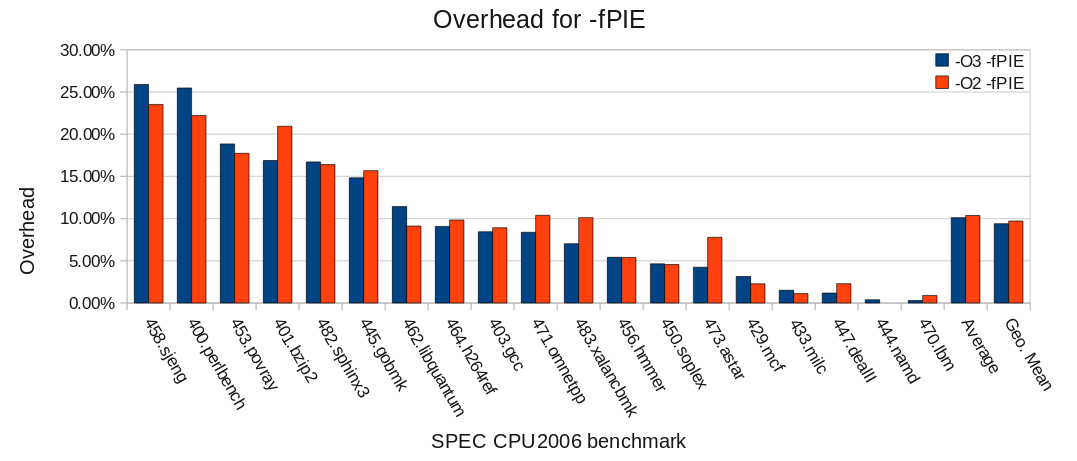
\includegraphics[width=\textwidth]{pie-cost}
\imagecredit{Payer, ``Too much PIE is bad for performance'', ETH Zurich Tech Report}
\end{frame}

\begin{frame}{position independence cost: Linux}
\begin{itemize}
    \item geometric mean of SPECcpu2006 benchmarks on x86 Linux
        \begin{itemize}
            \item with particular version of GCC, etc., etc.
        \end{itemize}
    \item 64-bit: 2-3\% (???)
        \begin{itemize}
        \item ``preliminary result''; couldn't find reliable published data
        \end{itemize}
    \item 32-bit: 9-10\%
    \item depends on compiler, \ldots
\end{itemize}
\end{frame}

\begin{frame}{position independence: deployment}
\begin{itemize}
    \item my laptop (64-bit Ubuntu 16.04): \textasciitilde 14\% of executables are PIE
    \item Ubuntu 16.10 (released 2016 Oct): enables PIE by default
        \begin{itemize}
            \item also Debian Stretch (late 2016), Fedora 23 (late 2015), \ldots
        \end{itemize}
    \item OS X enables PIE by default since 10.7 (despite perf. cost)
\end{itemize}
\end{frame}

\section{NX}

\againframe<2>{mappingList}

\begin{frame}[fragile,label=wxorx]{write XOR execute}
    \begin{itemize}
    \item many names:
    \begin{itemize}
        \item \verb|W^X| (write XOR execute)
        \item DEP (Data Execution Prevention)
        \item NX bit (No-eXecute) (hardware support)
        \item XD bit (eXecute Disable) (hardware support)
    \end{itemize}
    \item mark writeable memory as executable
    \item how will users insert their machine code?
        \begin{itemize}
        \item can only code in application + libraries
        \item a problem, right?
        \end{itemize}
    \end{itemize}
\end{frame}

\subsection{History of HW support}

\begin{frame}{hardware support for write XOR execute}
    \begin{itemize}
    \item everywhere today
    \item not historically common
    \item early x86: execute implied by read
    \item NX support added with x86-64 and around 2000 for x86-32
    \end{itemize}
\end{frame}

\begin{frame}{deliberate use of writeable code}
    \begin{itemize}
    \item ``just-in-time'' (JIT) compilers
        \begin{itemize}
        \item fast virtual machine/language implementations
        \end{itemize}
    \item some weird GCC features
    \item older ``signals'' on Linux
        \begin{itemize}
        \item OS wrote machine code on stack for program to run
        \end{itemize}
    \item couldn't even disable executable stacks without breaking applications
    \end{itemize}
\end{frame}

\begin{frame}{why doesn't W xor X solve the problem?}
    \begin{itemize}
    \item ASLR, stack canaries, etc. had performance penalty
        \begin{itemize}
        \item and failed if there was an information leak
        \end{itemize}
    \item W xor X is ``almost free'', keeps attacker from writing code?
    \item problem: useful machine code is in program already
        \begin{itemize}
        \item just need to find writable function pointer
        \end{itemize}
    \end{itemize}
\end{frame}

\begin{comment}
\begin{frame}{does ASLR+NX?}
    \begin{itemize}
    \item ASLR is ineffective due to information leaks
        \begin{itemize}
        \item if there's a memory error, pointer values are probably available
        \item any pointer value on stack --- all other addresses on stack
        \item any pointer value in library --- all other addresses in library
        \end{itemize}
    \item NX is ineffective in practice due to \myemph{return-oriented programming}
    \end{itemize}
\end{frame}
\end{comment}

\section{return-oriented programmming}

\begin{frame}{next topic: ROP}
    \begin{itemize}
    \item return-oriented programming
    \item AKA arc injection
    \item AKA return-to-libc
    \vspace{.5cm}
    \item find ``chain'' of machine code that does what you want
    \end{itemize}
\end{frame}

\begin{frame}{ROP case study}
    \begin{itemize}
    \item simple stack buffer overflow with write XOR execute
    \item stack canaries disabled
    \item ASLR disabled
        \begin{itemize}
        \item in practice --- rely on information disclosure bug
        \end{itemize}
    \end{itemize}
\end{frame}

\begin{frame}[fragile,label=vuln]{vulnerable application}
    \lstset{language=C,style=small}
\begin{lstlisting}
#include <stdio.h>

int vulnerable() {
    char buffer[100];
    gets(buffer);
}

int main(void) {
    vulnerable();
}
\end{lstlisting}
\end{frame}

\begin{frame}[fragile,label=vulnFunc]{vulnerable function}
    \lstset{language=myasm,style=small}
\begin{lstlisting}
0000000000400536 <vulnerable>:
  400536:       48 83 ec 78        sub    $0x78,%rsp
  40053a:       31 c0              xor    %eax,%eax
  40053c:       48 8d 7c 24 0c     lea    0xc(%rsp),%rdi
  400541:       e8 ca fe ff ff     callq  400410 <gets@plt>
  400546:       48 83 c4 78        add    $0x78,%rsp
  40054a:       c3                 retq   
\end{lstlisting}
    \begin{itemize}
        \item<2> buffer at \texttt{0xC} + stack pointer
        \item<2> return address at \texttt{0x78} + stack pointer
            \begin{itemize}
                \item = \texttt{0x6c} + buffer
            \end{itemize}
    \end{itemize}
\end{frame}

\begin{frame}[fragile,label=memoryLayout]{memory layout}
\lstset{
    language={},
    style=small,
    moredelim={**[is][\color{blue!70!black}]{~in~}{~end~}},
}
\begin{itemize}
    \item going to look for interesting code to run in libc.so
        \begin{itemize}
        \item implements gets, printf, etc.
        \end{itemize}
    \item loaded at address {\tt 0x2aaaaacd3000}
\end{itemize}
\end{frame}

\begin{frame}{our task}
    \begin{itemize}
    \item print out the message ``You have been exploited.''
    \item ultimately calling {\tt puts}
    \item which will be at address {\tt 0x2aaaaad42690}
    \end{itemize}
\end{frame}

\begin{frame}[fragile,label=shellcode]{shellcode}
\lstset{
    language=myasm,
    style=small,
    moredelim={**[is][\color{blue!70!black}]{~in~}{~end~}},
}
\begin{lstlisting}
        lea  string(%rip), %rdi
        mov  $0x2aaaaad42690, %rax /* puts */
        jmpq *(%rax)
string: .ascii "You have been exploited.\0"
\end{lstlisting}
    \begin{itemize}
        \item but --- can't insert code
        \item surely this code doesn't exist in libc already
        \item solution: find code for pieces
    \end{itemize}
\end{frame}

\begin{frame}[fragile,label=loadRDICode]{loading string into RDI}
\lstset{
    language=myasm,
    style=small,
    moredelim={**[is][\color{blue!70!black}]{~in~}{~end~}},
}
    \begin{itemize}
        \item can we even load a pointer to the string into {\tt \%rdi}?
        \item let's look carefully at code in {\tt libc.so}
    \end{itemize}
\begin{lstlisting}
2aaaaadfdc95:       48 89 e7              mov    %rsp,%rdi
2aaaaadfdc98:       ff d0                 callq  *%rax
\end{lstlisting}
    \begin{itemize}
        \item just need to get address of {\tt puts} into {\tt \%rax} before this
    \end{itemize}
\end{frame}

\begin{frame}[fragile,label=loadRDI]{load RDI}
\begin{tikzpicture}
% FIXME:
\tikzset{
    stackBox/.style={very thick},
    onStack/.style={thick},
}
\begin{scope}[xscale=0.75]
\draw[stackBox] (0, 2) rectangle (10, -3);
\draw[thick,-Latex] (-.25,-1) -- (-.25, 1) node [midway, above, sloped] {increasing addresses};
\node[at={(5, 2.1)},anchor=south] { highest address (stack started here)};
\node[at={(5, -3.1)},anchor=north] { lowest address (stack grows here)};

\draw[onStack] (0, -.25) rectangle (10, -1.25) node[midway,align=center,font=\small] (stackAddr)
     {return address for {\tt vulnerable}: \\ \only<2->{address of ``gadget''}};
\draw[onStack,fill=blue!20] (0, -1.25) rectangle (10, -2.25) node[midway,align=center,font=\small] {buffer (100 bytes)};

    \begin{visibleenv}<2->
\draw[onStack,fill=red!20,opacity=0.9] (0, -2.25) rectangle (10, -1.25) node[midway,align=center,font=\small,text=red!50!black] {unused junk};
\draw[onStack,fill=green!20,opacity=0.9] (0, -.25) rectangle (10, 1.0) node[midway,align=center,font=\small,text=red!50!black] {string pointed to by RDI};

\draw[-Latex,red,ultra thick,dashed] ([yshift=2.5mm]stackAddr.south east) -- ++(.25cm,0cm) |-
    (12, -1.25) node[align=left,right,font=\small] { {\tt mov \%rsp, \%rdi} \\ {\tt call *\%rax} };
\end{visibleenv}
\end{scope}
\end{tikzpicture}
\end{frame}

\begin{frame}[fragile,label=loadRAXCode]{loading puts addr. into RAX}
\lstset{
    language={},
    style=smaller,
    moredelim={**[is][\color{blue!70!black}]{~in~}{~end~}},
    moredelim={**[is][\color{red}\bfseries]{~hi~}{~end~}},
}
\begin{lstlisting}
2aaaaad06543:       e8 ~hi~58 c3~end~ fe ff          callq  2aaaaaaf48a0
\end{lstlisting}
\begin{itemize}
    \item {\tt 58 c3} can be interpreted another way: 
\begin{lstlisting}
2aaaaad06544:       58          popq %rax
2aaaaad06545:       c3          retq
\end{lstlisting}
    \item ``ret'' lets us \textbf{chain} this to execute \texttt{call} snippet next
\end{itemize}
\end{frame}

\begin{frame}[fragile,label=loadChain]{ROP chain}
\begin{tikzpicture}
% FIXME:
\tikzset{
    stackBox/.style={very thick},
    onStack/.style={thick},
    useLine/.style={very thick,blue,Latex-},
    useLineRet/.style={red,very thick,-Latex,dashed},
    gadgetBox/.style={blue,thick,text=black,draw,align=left,font=\small},
}
\begin{scope}[xscale=0.75]
\draw[stackBox] (0, 3) rectangle (10, -3);
\draw[thick,-Latex] (-.25,-1) -- (-.25, 1) node [midway, above, sloped] {increasing addresses};
\draw[onStack,fill=green!20,opacity=0.9] (0, 3.00) rectangle (10, 1.75) node[midway,align=center,font=\small] (theString)
     {string to print};
\draw[onStack,red] (0, 1.75) rectangle (10, .75) node[midway,align=center,font=\small] (gadgetTwo)
     {pointer to second gadget};
\draw[onStack,fill=green!20] (0, .75) rectangle (10, -.25) node[midway,align=center,font=\small] (putsAddr)
     {address of \texttt{puts} (popped from stack)};
\draw[onStack,red] (0, -.25) rectangle (10, -1.25) node[midway,align=center,font=\small] (stackAddr)
     {return address for {\tt vulnerable}: \\pointer to first gadget};
\draw[onStack,fill=blue!20] (0, -1.25) rectangle (10, -2.25) node[midway,align=center,font=\small] {buffer (100 bytes)};
\draw[onStack,fill=red!20,opacity=0.9] (0, -2.25) rectangle (10, -1.25) node[midway,align=center,font=\small,text=red!50!black] {unused junk};
        \draw[-Latex,red,ultra thick,dashed] (stackAddr.east) -- ++(3cm,0cm) 
        node[right,gadgetBox] (firstGad) { {\tt popq \%rax} \\ {\tt ret} };
        \draw[-Latex,red,ultra thick,dashed] (gadgetTwo.east) -- ++(3cm,0cm)
        node[right,gadgetBox] (secondGad) { {\tt mov \%rsp, \%rdi} \\ {\tt call *\%rax} };
    \begin{visibleenv}<2->
        \node[gadgetBox,dashed,below=1cm of firstGad] (realRet) {
            \texttt{ret} (in vulnerable)
        };
        \draw[useLineRet] ([xshift=1ex]realRet.west) -- ([xshift=-1ex,yshift=2ex]stackAddr.south east);
    \end{visibleenv}
    \begin{visibleenv}<3->
        \draw[useLine] ([yshift=.6em,xshift=1ex]firstGad.west) -- (putsAddr.east);
    \end{visibleenv}
    \begin{visibleenv}<4->
        \draw[useLineRet] ([yshift=-.6em,xshift=1ex]firstGad.west) -- ([xshift=-1ex,yshift=2ex]gadgetTwo.south east);
    \end{visibleenv}
    \begin{visibleenv}<4->
        \draw[useLine] ([yshift=.6em,xshift=1ex]secondGad.west) -- (theString.east);
    \end{visibleenv}
\end{scope}
\end{tikzpicture}
\end{frame}

% FIXME: demonstrating ROP exploit

\begin{frame}{demo}
\end{frame}

\begin{frame}{how did I find that?}
    \begin{itemize}
        \item no, I am not really good at looking at \texttt{objdump} output
        \item tools scan binaries for \textit{gadgets}
        \item one you'll use in upcoming homework
    \end{itemize}
\end{frame}

\begin{frame}{gadgets generally}
    \begin{itemize}
        \item bits of machine code that do work, then return or jump
        \item ``chain'' together, by having them jump to each other
        \item most common: find gadget ending with \texttt{ret}
            \begin{itemize}
            \item pops address of next gadget offs tack
            \end{itemize}
        \item can do pretty much anything
    \end{itemize}
\end{frame}

\begin{frame}{ROP and ASLR}
    \begin{itemize}
    \item find a pointer to known thing in libc (or other source of gadgets)
        \begin{itemize}
        \item e.g. information leak from use-after-free
        \end{itemize}
    \item use that to compute address of all gadgets
    \item then address randomization doesn't matter
    \end{itemize}
\end{frame}

\begin{frame}{ROP and write XOR execute}
    \begin{itemize}
    \item all the code we're running is supposed to be executed
    \item completely defeats write XOR execute
    \end{itemize}
\end{frame}

\begin{frame}{ROP and stack canaries}
    \begin{itemize}
    \item information disclosure reveals canary value if needed, still
    \item full stack canaries should reduce number of gadgets
        \begin{itemize}
        \item no real returns without canary checks
        \end{itemize}
    \item \ldots but typically only canaries if stack-allocated buffer
    \item and return opcodes within other instructions
    \end{itemize}
\end{frame}

\begin{frame}{ROP without a stack overflow (1)}
    \begin{itemize}
    \item e.g. VTable overwrite
    \item look for gadget(s) that set {\tt \%rsp}
    \item \ldots based on function argument registers/etc.
    \end{itemize}
\end{frame}

\begin{frame}{ROP without stack overflow (2)}
    \begin{itemize}
    \item example sequence from my libc:
        \begin{itemize}
            \item \texttt{push \%rdi; call *(\%rdx)}
            \item \texttt{pop \%rsp; ret}
        \end{itemize}
    \item set:
        \begin{itemize}
        \item overwritten vtable entry = first gadget
        \item arg 1: {\tt \%rdi} = desired stack pointer
        \item arg 3: {\tt \%rdx} = pointer to second gadget
        \end{itemize}
    \end{itemize}
\end{frame}

\begin{frame}{jump-oriented programming}
    \begin{itemize}
        \item just look for gadgets that end in \texttt{call} or \texttt{jmp}
        \item don't even need to set stack
        \item harder to find than \texttt{ret}-based gadgets
            \begin{itemize}
            \item but almost always as powerful as ret-based gadgets
            \end{itemize}
    \end{itemize}
\end{frame}

\begin{frame}{finding gadgets}
    \begin{itemize}
        \item find code segments of exectuable/library
        \item look for opcodes of arbitrary jumps:
            \begin{itemize}
            \item \texttt{ret}
            \item \texttt{jmp *register}
            \item \texttt{jmp *(register)}
            \item \texttt{call *register}
            \item \texttt{call *(register)}
        \end{itemize}
        \item disassemble starting a few bytes before
            \begin{itemize}
            \item invalid instruction? jump before ret? etc. --- discard
            \end{itemize}
        \item sort list
        \vspace{.5cm}
    \item \myemph{automatable}
    \end{itemize}
\end{frame}

\begin{frame}{finding gadgets: demo}
\end{frame}

\begin{frame}{programming with gadgets}
    \begin{itemize}
        \item can usually find gadgets to:
            \begin{itemize}
            \item pop from stack into argument register
            \item write register to memory location in another register
            \item clear a register
            \end{itemize}
        \item along with gadget for \texttt{syscall} (make OS call) --- can do anything
    \end{itemize}
\end{frame}

\begin{frame}{common, reusable ROP sequences}
    \begin{itemize}
        \item open a command-line --- what \texttt{ROPgadget} tool defaults to 
        \item make memory executable + jump
            \begin{itemize}
            \item generally: just do enough to ignore write XOR execute
            \end{itemize}
        \item often only depend on memory locations in shared library
    \end{itemize}
\end{frame}

\begin{frame}{ROP ideas}
    \begin{itemize}
        \item incidental \textit{existing} snippets of code
    \item chain together with non-constant jumps
        \begin{itemize}
        \item returns, function pointer calls, computed jumps
        \end{itemize}
    \item snippets form ``language''
        \begin{itemize}
        \item usually Turing-complete
        \end{itemize}
    \end{itemize}
\end{frame}
